\documentclass[journal,12pt,onecolumn]{IEEEtran}
\usepackage{graphicx, float}
\graphicspath{{figs/}}
\usepackage{multicol}
\usepackage{parskip}
\usepackage{titlesec}
\usepackage{color}
\usepackage{enumitem}
\usepackage{amsmath,amssymb,amsfonts,amsthm}
\usepackage{array}
\usepackage{booktabs}
\usepackage[table]{xcolor}
\usepackage{longtable}
\usepackage{gensymb}
\usepackage{cite}
\usepackage{algorithmic}
\usepackage{textcomp}
\usepackage{txfonts}
\usepackage{listings}
\usepackage{mathtools}
\usepackage{comment}
\usepackage{tkz-euclide}
\usepackage[breaklinks=true]{hyperref}
\usepackage{gvv}
\usepackage[latin1]{inputenc}
\usetikzlibrary{arrows.meta, positioning}
\usepackage{xparse}
\usepackage{calc}
\usepackage{multirow}
\usepackage{hhline}
\usepackage{ifthen}
\usepackage{lscape}
\usepackage{tabularx}
\usepackage{circuitikz}
\usepackage{tikz}
\newtheorem{problem}{Problem}
\newtheorem{theorem}{Theorem}[section]
\newtheorem{proposition}{Proposition}[section]
\newtheorem{lemma}{Lemma}[section]
\newtheorem{corollary}[theorem]{Corollary}
\newtheorem{example}{Example}[section]
\newtheorem{definition}[problem]{Definition}
\newcommand{\BEQA}{\begin{eqnarray}}
\newcommand{\EEQA}{\end{eqnarray}}
\theoremstyle{remark}
\title{Graduate Aptitude Test in Engineering 2025}
\author{EE25BTECH11025- Vishwambhar}

\begin{document}

\maketitle

\begin{enumerate}

\item Fish:Shoal::Lion:\dots\\
Select the correct option to complete the analogy
\begin{enumerate}
\begin{multicols}{4}
    \item Pride
    \item School
    \item Forest
    \item Series
\end{multicols}
\end{enumerate}
\hfill{(GATE PE 2025)}

\item Identify the grammatically correct sentence:
\begin{enumerate}
    \item It is I who am responsible for this fiasco.
    \item It is myself who is responsible for this fiasco.
    \item It is I who is responsible for this fiasco.
    \item It is I who is are responsible for this fiasco.
\end{enumerate}
\hfill{(GATE PE 2025)}

\item Two cars, P and Q, start from a point $X$ in India at 10 AM. Car P travels North with a speed of of 25 km/hr and car Q travels East with a speed of 30 km/hr. Car P travels continuously but car Q stops for some time after travelling for one hour. If both the cars are at the same distance from $X$ at 11:30 AM, for how long (in minutes) did car Q stop?
\begin{enumerate}
\begin{multicols}{4}
    \item 10
    \item 12
    \item 15
    \item 15
\end{multicols} 
\end{enumerate}
\hfill{(GATE PE 2025)}

\item The ceiling function of a real number $x$, denoted by $ce\brak{x}$, is defined as the smallest integer that is greater than or equal to $x$. Similarly, the floor function, denoted by $fl\brak{x}$, is defined as the largest integer that is smaller than or equal to $x$. Which one of the following statements is NOT correct for all possible values of $x$?
\begin{enumerate}
    \item $ce\brak{x}\geq x$
    \item $fl\brak{x}\leq x$
    \item $ce\brak{x}\geq fl\brak{x}$
    \item $fl\brak{x}< ce\brak{x}$
\end{enumerate}
\hfill{(GATE PE 2025)}

\item P and Q play chess frequently against each other. Of these matches, P has won 80\% of the matches, drawn 15\% of the matches and lost 5\% of the matches.\\
If they play 3 more matches, what is the probability of P winning exactly 2 of these 3 matches?
\begin{enumerate}
    \item $\frac{48}{125}$
    \item $\frac{16}{125}$
    \item $\frac{16}{25}$
    \item $\frac{25}{48}$
\end{enumerate}
\hfill{(GATE PE 2025)}

\item Identify the option that has the most appropriate sequence such that a coherent paragraph is formed:\\
P. At once, without thinking much, people rushed towards the city in hordes with the sole aim of grabbing as much gold as they could.\\
Q. However, little did they realize about the impending hardships they would have to face on their way to the city: miles of mud, unfriendly forests, hungry beasts and inimical local lords - all of which would reduce their chances of getting gold to almost zero.\\
R. All of them thought that easily they could lay their hands on gold and become wealthy overnight.
S. About a hundred years ago, the news that gold had been discovered in Kolar spread like wildfire and the whole State was in raptures.
\begin{enumerate}
    \item P $\rightarrow$ Q $\rightarrow$ R $\rightarrow$ S
    \item Q $\rightarrow$ S $\rightarrow$ R $\rightarrow$ P
    \item S $\rightarrow$ Q $\rightarrow$ P $\rightarrow$ R
    \item S $\rightarrow$ P $\rightarrow$ R $\rightarrow$ Q
\end{enumerate}
\hfill{(GATE PE 2025)}

\item If HIDE and CAGE are coded as 19-23-7-11 and 5-2-17-11 respectively, them what is the code for HIGH
\begin{enumerate}
    \item 5-17-1-2
    \item 17-19-13-17
    \item 13-3-1-2
    \item 19-23-17-19
\end{enumerate}
\hfill{(GATE PE 2025)}

\item The given figure is reflected about the horizontal dashed line and then rotated clockwise by $90\degree$ about an axis perpendicular to the plane of the figure.\\
Which one of the following options correctly shows the resultant figure?\\
Note: The figures shown are representative.
\begin{figure}[H]
    \centering
    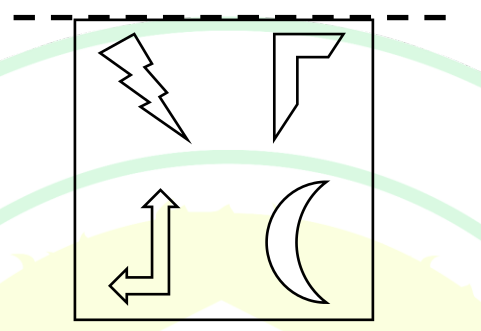
\includegraphics[width=0.3\columnwidth]{25Q8.png}
    \caption{}
    \label{fig:placeholder}
\end{figure}
\begin{enumerate}
    \item \begin{figure}[H]
    \centering
    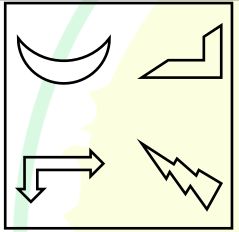
\includegraphics[width=0.15\columnwidth]{25Q8_1.png}
    \caption{}
    \label{fig:placeholder}
\end{figure}
    \item \begin{figure}[H]
    \centering
    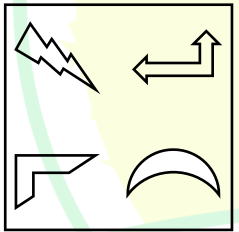
\includegraphics[width=0.15\columnwidth]{25Q8_2.png}
    \caption{}
    \label{fig:placeholder}
\end{figure}
    \item \begin{figure}[H]
    \centering
    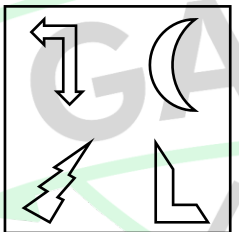
\includegraphics[width=0.15\columnwidth]{25Q8_3.png}
    \caption{}
    \label{fig:placeholder}
\end{figure}
    \item \begin{figure}[H]
    \centering
    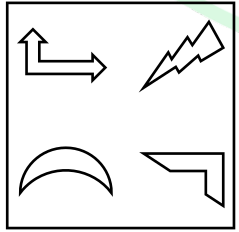
\includegraphics[width=0.15\columnwidth]{25Q8_4.png}
    \caption{}
    \label{fig:placeholder}
\end{figure}
\end{enumerate}
\hfill{(GATE PE 2025)}

\item Which one of the following options has the correct sequence of objects arranged in the increasing number of mirror lines (lines of symmetry)?
\begin{enumerate}
    \item Circle; Square; Equilateral triangle; Isosceles triangle
    \item Isosceles triangle; Equilateral triangle; Square; Circle
    \item Equilateral triangle; Isosceles triangle; Square; Circle
    \item Isosceles triangle; Square; Equilateral triangle; Circle
\end{enumerate}
\hfill{(GATE PE 2025)}

\item A final year student appears for placement interview in two companies, S and T. Based on her interview performance, she estimates the probability of receiving job offers from companies S and T to be 0.8 and 0.6, respectively. Let $p$ be the probability that she receives job offers from both the companies. Select the most appropriate option.
\begin{enumerate}
    \item $0 \leq p \leq 0.2$
    \item $0.4 \leq p \leq 0.6$
    \item $0.2 \leq p \leq 0.4$
    \item $0.6 \leq p \leq 1.0$
\end{enumerate}
\hfill{(GATE PE 2025)}

\item Four fair coins are tossed simultaneously. The probability that at least one tail turns up is
\begin{enumerate}
\begin{multicols}{4}
    \item $\frac{1}{16}$
    \item $\frac{15}{16}$
    \item $\frac{7}{8}$
    \item $\frac{1}{2}$
\end{multicols}
\end{enumerate}
\hfill{(GATE PE 2025)}

\item Let $\vec{A}=2\vec{i}-\vec{j}+\vec{k}$ and $\vec{B}=\vec{i}+\vec{j}$, where $\vec{i},\vec{j},$ and $\vec{k}$ are unit vectors. The projection of $\vec{B}$ on $\vec{A}$ is
\begin{enumerate}
\begin{multicols}{4}
    \item $\frac{1}{\sqrt{12}}$
    \item $\frac{1}{\sqrt{6}}$
    \item $\sqrt{6}$
    \item $\frac{1}{\sqrt{2}}$
\end{multicols}
\end{enumerate}
\hfill{(GATE PE 2025)}

\item The value $\lim\limits_{x \to \dfrac{\pi}{2}}\brak{\dfrac{\cos{x}}{x-\frac{\pi}{2}}}$
\begin{enumerate}
\begin{multicols}{4}
    \item 1
    \item -1
    \item 0
    \item $\pi$
\end{multicols}
\end{enumerate}
\hfill{(GATE PE 2025)}


\item Which ONE of the following CANNOT be obtained from pressure transient analysis in well testing?
\begin{enumerate}
    \item Formation damage
    \item Average reservoir pressure
    \item Solution gas-oil ratio
    \item Drainage pore volume
\end{enumerate}
\hfill{(GATE PE 2025)}

\item The primary objective of the electrostatic grid in electrostatic heater-treater used in crude oil processing is to
\begin{enumerate}
    \item separate sand particles.
    \item promote coalescence of water droplets.
    \item generate electrical energy from the kinetic energy of the feed.
    \item prevent corrosion by the cathodic protection.
\end{enumerate}
\hfill{(GATE PE 2025)}

\item The maximum Polished Rod Load (PRL) in the operation of the sucker rod pump is observed near the
\begin{enumerate}
    \item top of the stroke and the traveling valve is open
    \item top of the stroke and the traveling valve is closed
    \item bottom of the stroke and the traveling valve is open
    \item bottom of the stroke and the traveling valve is closed.
\end{enumerate}
\hfill{(GATE PE 2025)}

\item Four curves designated as I, II, III, and IV are shown in the figure. $P_b$ is the bubble point pressure of a crude oil at the given temperature.\\
Which ONE of the following options correctly depicts the solubility of asphaltene $q_b$ in the crude oil with pressure $\brak P$ at a given temperature?
\begin{figure}[H]
    \centering
    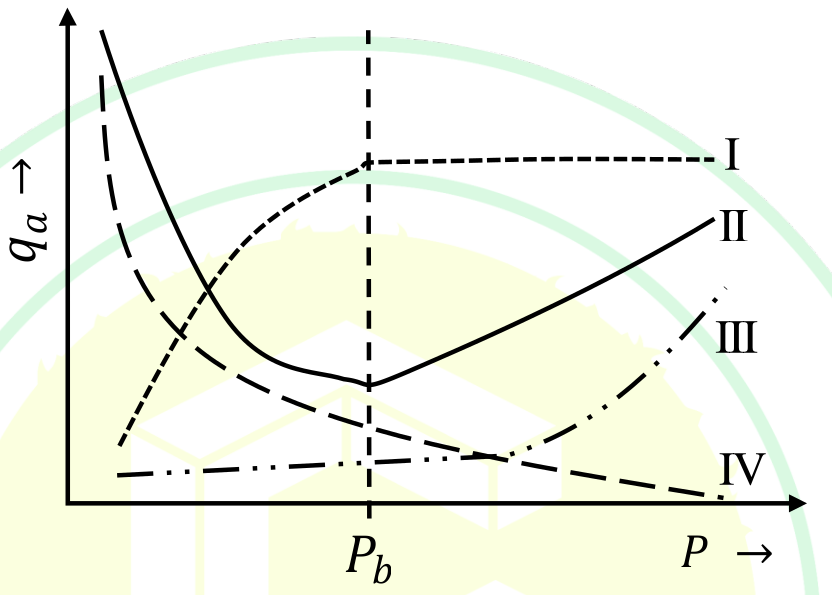
\includegraphics[width=0.4\columnwidth]{25Q17.png}
    \caption{}
    \label{fig:placeholder}
\end{figure}
\begin{enumerate}
\begin{multicols}{4}
    \item I
    \item II
    \item III
    \item IV
\end{multicols}
\end{enumerate}
\hfill{(GATE PE 2025)}

\item $C_1, C_2$ and $C_3$ are the Dietz shape factors of three reservoirs with circular, square, and rectangular shape of drainage area, respectively. The well is located at the geometric center of the reservoir.\\
Which ONE of the following options is CORRECT about the shape factors?
\begin{enumerate}
    \item $C_3<C_2<C_1$
    \item $C_2<C_1<C_3$
    \item $C_1<C_2=C_3$
    \item $C_1=C_2<C_3$
\end{enumerate}
\hfill{(GATE PE 2025)}

\item Four curves designated as I, II, III, and IV are shown in the figure. $q_f$ is the bottomhole oil flow rate, q s is the surface oil flow rate, and $B_o$ is the oil formation volume factor.\\
Which ONE of the following curves depicts the minimum wellbore storage effect?
\begin{figure}[H]
    \centering
    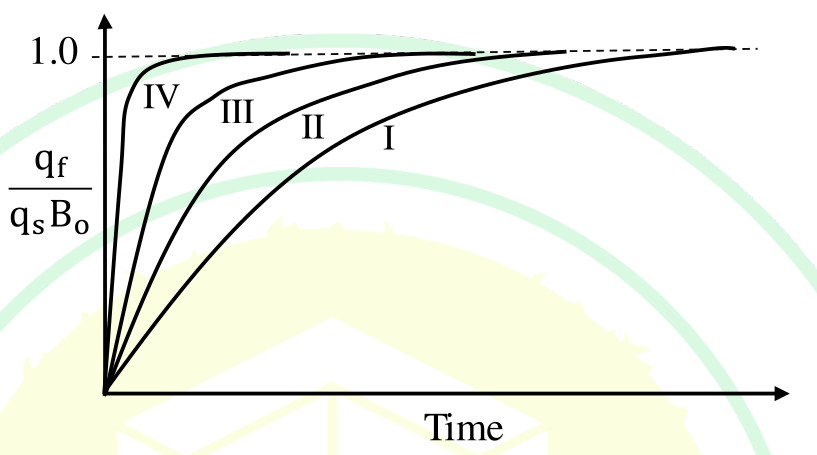
\includegraphics[width=0.4\columnwidth]{25Q19.png}
    \caption{}
    \label{fig:placeholder}
\end{figure}
\begin{enumerate}
\begin{multicols}{4}
    \item I
    \item II
    \item III
    \item IV
\end{multicols}
\end{enumerate}
\hfill{(GATE PE 2025)}

\item Match the entries in GROUP I with the entries in GROUP II.\\

\begin{tabular}[12pt]{|c|c|}
\hline
\textbf{GROUP I}&\textbf{GROUP II}\\
\hline
(P)Liquid hold-up&(I)Water removal\\
\hline
(Q)Liquid carryover&(II) Free gas escaping with liquid phase\\
\hline
(R)Gas blowby&(III) Free liquid escaping with gas phase\\
\hline
(S)Gas dehydration&(IV) Fraction of pipe volume occupied by liquid\\
\hline
\end{tabular}
\begin{enumerate}
    \item P-III;Q-IV;R-I;S-II
    \item P-IV;Q-III;R-II;S-I
    \item P-I;Q-II;R-IV;S-III
    \item P-IV;Q-II;R-III;S-I
\end{enumerate}
\hfill{(GATE PE 2025)}

\item Which ONE of the following rocks shows the highest reading in the natural gamma ray log?
\begin{enumerate}
\begin{multicols}{4}
    \item Dolomite
    \item Anhydrite
    \item OIl shade
    \item Limestone
\end{multicols}
\end{enumerate}
\hfill{(GATE PE 2025)}

\item Crude oil denser than pure water has the API gravity
\begin{enumerate}
    \item less than $10\degree$
    \item between $10\degree$ and $20\degree$
    \item between $20\degree$ and $60\degree$
    \item more than $60\degree$
\end{enumerate}
\hfill{(GATE PE 2025)}

\item Which ONE of the following options is CORRECT in relation to the standard drill pipe?
\begin{enumerate}
    \item Nominal weight is equal to the actual weight
    \item Nominal weight is less than the actual weight
    \item Nominal weight is greater than the actual weight.
    \item Nominal weight is twice the actual weight.
\end{enumerate}
\hfill{(GATE PE 2025)}

\item Four different multilateral well patterns (Forked, Branched, Dual opening and Splayed) are shown in the figure.\\
Which ONE of the following options correctly identifies the multilateral well patterns?
\begin{figure}[H]
    \centering
    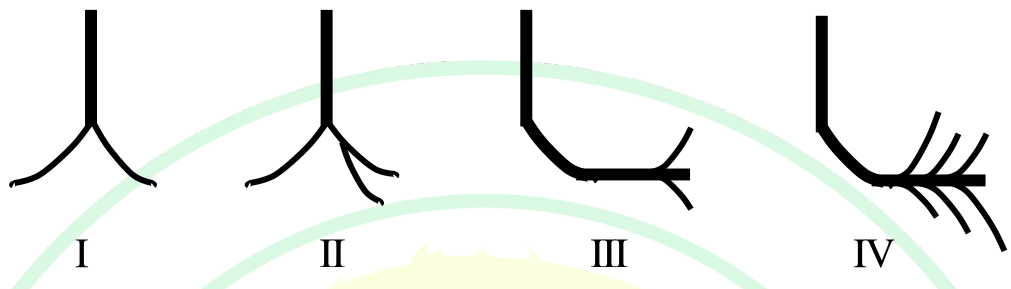
\includegraphics[width=0.4\columnwidth]{25Q24.png}
    \caption{}
    \label{fig:placeholder}
\end{figure}
\begin{enumerate}
    \item I-Forked; II-Branched; III-Dual opening; IV- Splayed
    \item I-Dual opening; II-Branched; III-Forked; IV- Splayed
    \item I-Dual opening; II-Splayed; III-Forked; IV- Branched
    \item I-Branched; II-Dual opening; III-Splayed; IV- Forked
\end{enumerate}
\hfill{(GATE PE 2025)}

\item For a hydrocarbon reservoir, the following parameters are used in the general material balance equation (MBE).\\
$N$= Initial (original) oil in place, stb\\
$G$= Initial volume of gas cap, scf\\
$m$ = Ratio of initial volume of gas cap to volume of oil initial in place, rb/rb\\
$S_{wi}$ = Initial water saturation\\
$S_{oi}$  = Initial oil saturation\\
$B_{oi}$= Initial oil formation volume factor, rb/stb\\
$B_{gi}$ = Initial gas formation volume factor, rb/scf\\
The total pore volume (in rb) of the reservoir is
\begin{enumerate}
    \item $\frac{GB_{gi}\brak{1+m}}{1-S_{oi}}$
    \item $\frac{NB_{oi}\brak{1-m}}{1-S_{oi}}$
    \item $\frac{GB_{oi}\brak{1+m}}{1-S_{wi}}$
    \item $\frac{GB_{gi}\brak{1-m}}{1-S_{wi}}$
\end{enumerate}
\hfill{(GATE PE 2025)}

\item Which of the following statement(s) is/are CORRECT?
\begin{enumerate}
    \item Gradient of temperature is a vector.
    \item Gradient of pressure is a vector.
    \item Divergence of velocity is a vector.
    \item Gradient of velocity is a scalar.
\end{enumerate}
\hfill{(GATE PE 2025)}

\item Which of the following statement(s) is/are CORRECT about the chemicals used for the processing of sour crude oil and natural gas?
\begin{enumerate}
    \item Amine solutions cannot be regenerated after removal of H$_2$S from natural gas.
    \item Amine solutions in liquid form absorb H$_2$S from natural gas.
    \item Glycols become corrosive in the presence of oxygen.
    \item Iron sponges cannot be used for H$_2$S removal.
\end{enumerate}
\hfill{(GATE PE 2025)}

\item Consider the following diffusivity equation for the radial flow of a fluid in an infinite and homogeneous reservoir.\\
$\frac{1}{r}\frac{\partial}{\partial r}\brak{r\frac{\partial P}{\partial r}}=\frac{1}{\eta}\frac{\partial P}{\partial t}$
where, $P$ denotes pressure, $r$ is the radial distance from the centre of the wellbore,$t$ denotes time, and, $\eta$ is the diffusivity constant. The initial pressure of the reservoir
is $P_i$.
The condition(s) used in the derivation of analytical solution of the above equation for pressure transient analysis in an infinite acting reservoir is/are:
\begin{enumerate}
    \item At time $t=0, P=P_i$ for all $r$.
    \item Wellbore is treated as a line source.
    \item As $r\xrightarrow[]{} \infty$, $P\xrightarrow[]{} P_i$ for all $t$.
    \item At any radius $r$ and time $t$, the pressure gradient $\frac{\partial P}{\partial r}$ is constant.
\end{enumerate}
\hfill{(GATE PE 2025)}

\item Which of the following offshore drilling platform(s) has/have legs on the seabed?
\begin{enumerate}
    \item Jack up
    \item Tension leg
    \item Concrete gravity
    \item Semi-submersible
\end{enumerate}
\hfill{(GATE PE 2025)}

\item Which of the following statement(s) is/are CORRECT about polymer flooding?
\begin{enumerate}
    \item Viscous fingering in the reservoir decreases.
    \item Viscosity of the displaced fluid increases.
    \item Mobility of the displacing fluid increases
    \item Mobility ratio decreases.
\end{enumerate}
\hfill{(GATE PE 2025)}

\item The hoisting system of a drilling rig contains seven ideal sheaves with hook load of $3.0 \times 10^5$kg.
The static derrick load is \dots $\times 10^5$ kg (rounded off to one decimal place)

\hfill{(GATE PE 2025)}

\item The product of the roots of the equation $x^4+1=0$ is \dots (answer in integer)

\hfill{(GATE PE 2025)}

\item Reservoir Quality Index (RQI) based on Kozeny-Carman equation as a function $\brak{f}$ of permeabilty ($k$ in m$D$) and porosity ($\phi$ in fraction) is given by\\
RQI = C$f\brak{k.\phi}$\\
where, Cis a constant with a value of 0.0314.\\
If a carbonate reservoir of 152 m$D$ and the porosity of 0.18, then the RQI is \dots $\mu m$(rounded off to two decimal places)\\

\hfill{(GATE PE 2025)}

\item The ratio of number of production to injection wells for a regular Seven-Spot pattern is \dots(rounded off to one decimal place).\\

\hfill{(GATE PE 2025)}

\item Natural gas is produced at a flow rate of 2 MMscf/day at the wellhead having temperature and pressure of $560\degree$R and 200 psi, respectively. The apparent molecular weight and the compressibility factor ($Z$) of the gas are estimated to be
20 g/g-mole and 0.8, respectively, at wellhead conditions.\\
The gas formation volume factor ($B_g$) at the wellhead
is \dots$\times10^{-2}$ ft$^3$/scf (rounded off to one decimal place)\\

\hfill{(GATE PE 2025)}

\item If $\frac{dy}{dx}+y=x$, and $y\brak{0}=0$, then the value of $y\brak{1}$ is 
\begin{enumerate}
\begin{multicols}{4}
    \item $e$
    \item $\frac{1}{e}$
    \item $1$
    \item $-1$
\end{multicols}
\end{enumerate}
\hfill{(GATE PE 2025)}

\item Let $f\brak{x}=ln x$. The first derivative $f'(x)$ is to be calculated at $x=1$ using numerical differentiation. $f'(1)$ is calculated using first order forward difference $\brak{f'_{FD}}$, first order backward difference $\brak{f'_{BD}}$, and second order central difference $f'_{CD}$, using interval width h = 0.1.\\
The CORRECT order of the values of $\brak{f'_{FD}}$, $\brak{f'_{BD}}$, and $\brak{f'{CD}}$ is
\begin{enumerate}
    \item $f'_{FD}>f'_{CD}>f'_{BD}$
    \item $f'_{CD}>f'_{BD}>f'_{FD}$
    \item $f'_{BD}>f'_{FD}>f'_{CD}$
    \item $f'_{BD}>f'_{CD}>f'_{Fd}$
\end{enumerate}
\hfill{(GATE PE 2025)}

\item Three different pressure profiles are shown in the figure. CSD is Casing Setting Depth.
Match the entries in \textbf{GROUP I} with the entries in \textbf{GROUP II}\\

\begin{tabular}[12pt]{|c|c|}
\hline
\textbf{GROUP I}&\textbf{GROUP II}\\
\hline
(P)Profile 1&(I) Reduced wellbore integrity due to weak formation\\
\hline
(Q)Profile 2&(II) Reduced wellbore integrity due to weak casing\\
\hline
(R)Profile 3&(III) Full wellbore integrity\\
\hline
\end{tabular}
\begin{figure}[H]
    \centering
    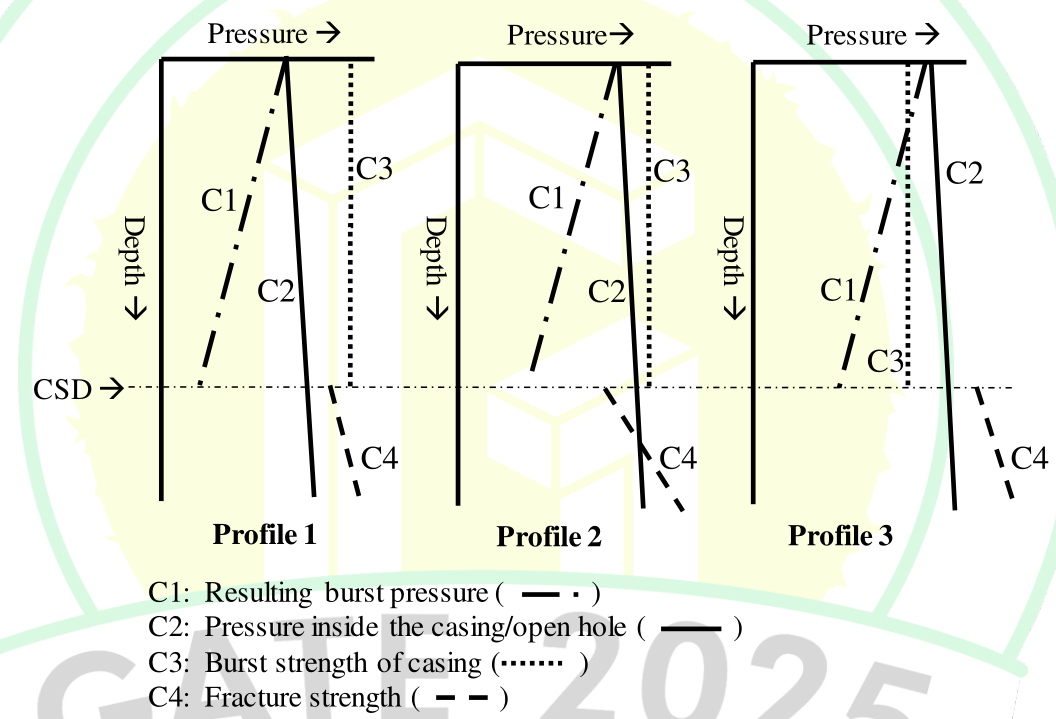
\includegraphics[width=0.5\columnwidth]{25Q38.png}
    \caption{}
    \label{fig:placeholder}
\end{figure}
\begin{enumerate}
    \item P-I;Q-II;R-III
    \item P-II;Q-III;R-I
    \item P-III;Q-I;R-II
    \item P-II;Q-I;R-III
\end{enumerate}
\hfill{(GATE PE 2025)}

\item Match the well logging methods in \textbf{GROUP I} with their corresponding measured parameters in \textbf{GROUP II}\\

%39
\begin{tabular}{|c|c|c|}
\hline
\textbf{Outcomes} & \textbf{Probability} & \textbf{Reward/Win (in INR)} \\
\hline
I   & 0.2 & 25 \\
\hline
II  & 0.3 & 50 \\
\hline
III & 0.5 & 100 \\
\hline
\end{tabular}

\begin{enumerate}
    \item P-IV;Q-I;R-II;S-III
    \item P-II;Q-IV;R-I;S-III
    \item P-II;Q-III;R-IV;S-I
    \item P-III;Q-IV;R-I;S-II
\end{enumerate}
\hfill{(GATE PE 2025)}

\item A drilling fluid with time-dependent rheology is used for the rotary drilling of a reservoir. The following equation describes the dependence of shear stress $\brak{\tau}$ on
shear rate $\brak{\gamma}$.\\
$\tau+\frac{\mu_o}{\alpha}\frac{d\tau}{dt}=\mu_o\gamma$
where, $\mu_o$ and $\alpha$ are constants.\\
If the rotation of the drill pipe is stopped at time $t=0$, then the relaxation behavior of the fluid stress with time is
\begin{enumerate}
    \item $\tau \propto e^{-\frac{\mu_ot}{\alpha}}$
    \item $\tau \propto e^{\frac{\mu_ot}{\alpha}}$
    \item $\tau \propto e^{-\frac{\alpha t}{\mu_o}}$
    \item $\tau \propto e^{\frac{\alpha t}{\mu_o}}$
\end{enumerate}
\hfill{(GATE PE 2025)}

\item Classification of kerogen is based on the relative amount of Carbon (C), Hydrogen (H) and Oxygen (O).\\
Which ONE of the following options is CORRECT about Type II kerogen?
\begin{enumerate}
    \item It is low in aliphatic compounds and H:C ratio < 0.84.
    \item It is rich in aliphatic compounds and H:C ratio < 0.84.
    \item It is low in aliphatic compounds and H:C ratio > 1.0.
    \item It is rich in aliphatic compounds and H:C ratio > 1.0.
\end{enumerate}
\hfill{(GATE PE 2025)}

\item The eigenvalues of the matrix $\myvec{3&-1&1\\
-1&5&-1\\
1&-1&3
}$ are $\lambda_1,\lambda_2$ and $\lambda_3$.\\
The value of $\lambda_1\lambda_2\lambda_3\brak{\lambda_1+\lambda_2+\lambda_3}$ is
\begin{enumerate}
\begin{multicols}{4}
    \item 11
    \item 45
    \item 396
    \item 495
\end{multicols}
\end{enumerate}
\hfill{(GATE PE 2025)}


\item A stationary tank is cylindrical in shape with two hemispherical ends and is horizontal, as shown in the figure. $R$ is the radius of the cylinder as well as of the hemispherical ends. The tank is half filled with an oil of density $\rho$ and the rest of the space in the tank is occupied by air. The air pressure, inside the tank as well as outside it, is atmospheric. The acceleration due to gravity $\brak{g}$ acts vertically
downward.\\
The net horizontal force applied by the oil on the right hemispherical end (shown by the bold outline in the figure) is
\begin{figure}[H]
    \centering
    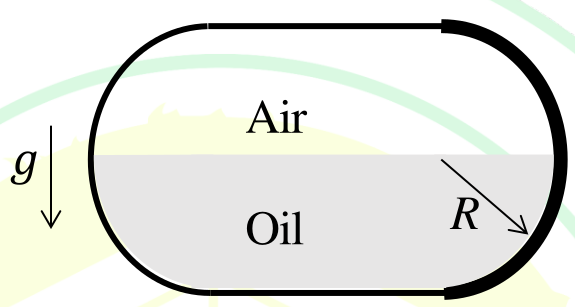
\includegraphics[width=0.5\columnwidth]{25Q43.png}
    \caption{}
    \label{fig:placeholder}
\end{figure}
\begin{enumerate}
\begin{multicols}{4}
    \item $\frac{1}{2}\rho g R^3$
    \item $\frac{2}{3}\rho g R^3$
    \item $\frac{3}{4}\rho g R^3$
    \item $\frac{1}{3}\rho g R^3$
\end{multicols}
\end{enumerate}
\hfill{(GATE PE 2025)}

\item If a function $f\brak{x}$ is continuous in the closed interval $\sbrak{a,b}$ and the first derivative $f'\brak{x}$ exists in the open interval $\brak{a,b}$, then according to the Lagrange's mean value theorem\\
$\frac{f\brak{b}-f\brak{a}}{b-a}$\\
If $a=0, b=1.5$, and $f\brak{x}=x\brak{x-1}\brak{x-2}=f'\brak{c}$, then the value(s) of $c$ in $$\sbrak{a,b}$$ is/are
\begin{enumerate}
\begin{multicols}{4}
    \item 0.50
    \item 0.75
    \item 1.00
    \item 1.50
\end{multicols}
\end{enumerate}
\hfill{(GATE PE 2025)}

\item Which of the following logging tool(s) underestimate(s) porosity in a gas-bearing formation?
\begin{enumerate}
    \item Neutron log
    \item Nuclear Magnetic Resonance (NMR) log
    \item Sonic log
    \item Density log
\end{enumerate}
\hfill{(GATE PE 2025)}


\item The effect of pressure on various properties of black oil is shown in the figure. The bubble point pressure is $P_b$ .\\
\begin{figure}[H]
    \centering
    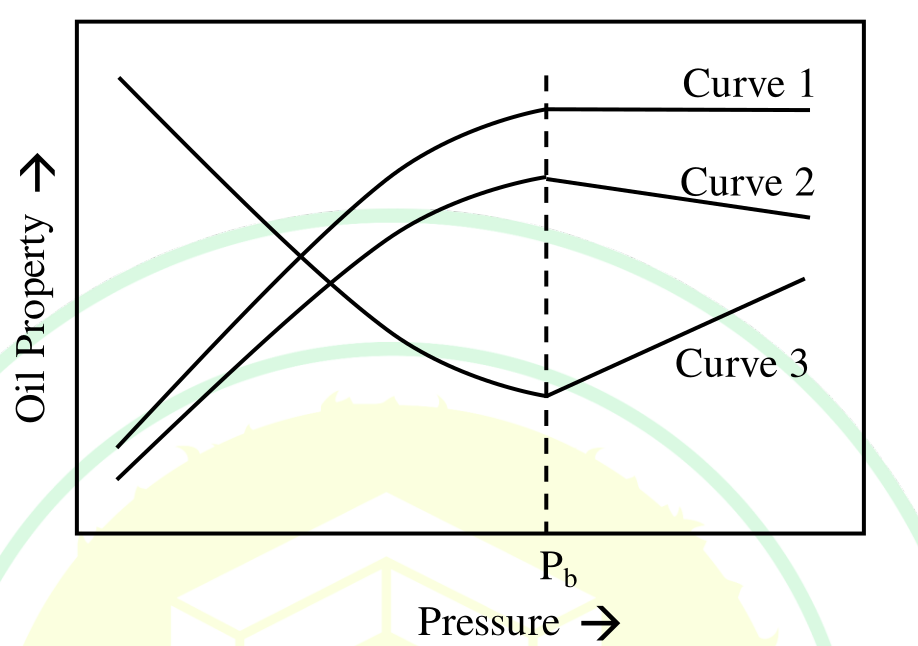
\includegraphics[width=0.5\columnwidth]{25Q46.png}
    \caption{}
    \label{fig:placeholder}
\end{figure}
Which of the following option(s) is/are CORRECT?
\begin{enumerate}
    \item Curve 1 represents solution gas-oil ratio.
    \item Curve 2 represents oil viscosity.
    \item Curve 3 represents oil formation volume factor.
    \item Curve 3 represents oil density.
\end{enumerate}
\hfill{(GATE PE 2025)}

\item Which of the following definition(s) related to fire and explosion is/are CORRECT?
\begin{enumerate}
    \item Fire point is the lowest temperature at which the vapour above a liquid will continue to burn once ignited
    \item Deflagration is the explosion in which the reaction front moves at a speed greater than the speed of sound in the unreacted medium.
    \item Detonation is the explosion in which the reaction front moves at a speed less than the speed of sound in the unreacted medium.
    \item Flash point of a liquid is the lowest temperature at which it gives enough vapour to form an ignitable mixture with air.
\end{enumerate}
\hfill{(GATE PE 2025)}


\item Which of the following option(s) is/are CORRECT for well testing analysis of a reservoir?
\begin{enumerate}
    \item Permeability, skin and reservoir geometry are calculated using data from pseudo steady state
    \item Permeability, skin and reservoir geometry are calculated using data from transient state
    \item Reservoir geometry is calculated using data from pseudo steady state.
    \item Absolute open flow potential is calculated from back pressure test for a gas well.
\end{enumerate}
\hfill{(GATE PE 2025)}

\item In a capillary rise experiment with a capillary tube of length $l_1$, water rises to a height h such that $h<l_1$.\\
If the capillary tube is cut to a length $l_2$ such that $l_2<h$, and the experiment is repeated, which of the following statements is/are CORRECT?
\begin{enumerate}
    \item Water overflows from the top of the tube
    \item Water does not overflow from the top of the tube
    \item At equilibrium, radius of curvature of meniscus are same in both the experiments..
    \item At equilibrium, radius of curvature of meniscus are different in both the experiments
\end{enumerate}
\hfill{(GATE PE 2025)}

\item The formation resistivity factor ($F$) is related to the formation porosity ($\phi$) in a water-bearing carbonate formation by the following correlation\\
$F=0.9\phi^2$\\
where $\phi$ is in fraction. The resistivity of the invaded zone of the formation obtained by the Microspherically Focused Log (MSFL) is 4.5 $\ohm m$, and the resistivity of the mud-filtrate is $0.05 \ohm m$.\\
The formation porosity is \dots \% (rounded off to one decimal place).

\hfill{(GATE PE 2025)}

\item The drainage oil-water capillary pressure data for a core retrieved from a homogeneous isotropic reservoir is listed in the table. The reservoir top is at 4000 ft from the surface and the water-oil contact (WOC) depth is at 4100 ft.\\
\begin{tabular}[12pt]{|c|c|}
\hline
\textbf{Water saturation (\%)}&\textbf{Capillary pressure (psi)}\\
\hline
100.0&0.0\\
\hline
100.0&5.5\\
\hline
99.0&5.6\\
\hline
89.2&6.4\\
\hline
81.8&6.9\\
\hline
44.2&11.2\\
\hline
29.7&17.1\\
\hline
25.1&36.0\\
\hline
\end{tabular}\\
Assume the densities of water and oil at reservoir conditions are 1.04 g/cc and 0.84 g/cc, respectively. The acceleration due to gravity is 980 cm/$s^2$. The interfacial tension between oil and water is 35 dynes/cm and the contact angle is $0\degree$.\\
The depth of free-water level (FWL) is at \dots ft (rounded off to one decimal place).\\
(Use: 1 psi = 68950 dynes/$cm^2$ ; 1 ft = 30.5 cm)

\hfill{(GATE PE 2025)}

\item The porosity of a formation with matrix density of 2.65 g/cc and fluid density of 1.0 g/cc is 0.15. The formation has shear modulus of 30 GPa and bulk modulus of 36 GPa.\\
The compressional wave velocity in the formation is \dots$\times 10^3$(rounded off to two decimal places).

\hfill{(GATE PE 2025)}

\item The hydrostatic pressure gradient in a vertical well drilled in a relaxed depositional basin is 0.452 psi/ft. Assume that the gradient of effective horizontal stress with depth is constant in the drilling zone and has a value of $9.96\times 10^{-2}$. The casing shoe is at 4000 ft depth.\\
While drilling the bore hole below the casing shoe with 10 ppg mud, the maximum allowed standpipe pressure is \dots psi (rounded off to one decimal place).\\
(Note: 1 ppg mud is equivalent to 0.052 psi/ft.)

\hfill{(GATE PE 2025)}


\item A vertical well is drilled up to a depth of 4000 ft. Further drilling starts with 10 ppg of fresh mud and 50000 lbf weight on bit (WOB). An equivalent circulation density (ECD) of 10.75 ppg was recorded. The total circulation pressure loss is estimated to be 110 psi. The still density is 65.5 ppg.\\
The decrease in hook load is \dots lbf (rounded off to one decimal place).\\
(Note: 1 ppg mud is equivalent to 0.052 psi/ft.)

\hfill{(GATE PE 2025)}

\item A horizontal well is planned with two radial sections to land the target at an angle of $90\degree$. The total vertical depth (TVD) between the surface and the target is 8000 ft. The buildup rate is $6\degree$ per 100 ft in the first section and $9\degree$ per 100 ft in the second section. The total angle built by the second section is $30\degree$.\\
The distance of the first kickoff point from the surface is \dots ft (rounded off to one decimal place).

\hfill{(GATE PE 2025)}

\item The laboratory analysis data obtained from the core is as follows:\\
Weight of clean dry core in air = 30 g\\
Weight of core completely saturated with oil = 32 g\\
Weight of saturated core completely immersed in oil = 24 g\\
If the density of oil used for saturation of core during the experiment is 0.88 g/cc, then the effective porosity of the core is \dots \% (rounded off to two decimal places).

\hfill{(GATE PE 2025)}

\item The Buckley Leverett frontal advance theory is employed to evaluate the performance of the water flooding operation in a horizontal reservoir. 
The following data are given:\\
Cross-sectional flow area = 40000 $ft^2$\\
Payzone thickness = 20 ft\\
Porosity = 20\%\\
Water injection rate = 1000 rb/day\\
Distance between injection and production well = 1000 ft\\
Cumulative pore volume of water injected (PVWI) at breakthrough = 0.5\\
The time of breakthrough is \dots days (rounded off to one decimal place).
(Use: 1 acre = 43560 $ft^2$ and 1 bbl = 5.615 $ft^3$)

\hfill{(GATE PE 2025)}

\item A hydraulically fractured vertical well has fracture permeability of 4000 mD, reservoir permeability of 80 mD, fracture width of 0.12 in, and fracture half-length of 1000 ft.
Dimensionless fracture conductivity is $\dots \times 10^{-4}$  (rounded off to one decimal place).

\hfill{(GATE PE 2025)}

\item An electrical submersible pump is to be installed to lift oil of $30\degree$ API in a 10000 ft deep well. The oil formation volume factor ($B_o$) is 1.25 rb/stb. The desired flow rate
is 8000 stb/day. Minimum suction pressure of the chosen pump is 200 psi. Inflow performance relationship shows a flowing bottomhole pressure of 2820 psi at the desired flow rate.\\
Assuming casing pressure and weight of the gas in the annulus to be negligible, the minimum pump setting depth is \dots ft (rounded off to one decimal place).

\hfill{(GATE PE 2025)}


\item Log-log plot of pressure drop ($\triangle p$) versus time ($t$) obtained using well test data is matched with one of the Grigarten type curves. Thereafter, a point on the type curve
is chosen with $P_D=10$ and $t_D/C_D$, where $P_D,t_D$ and $C_D$ are dimensionless pressure, dimensionless time, and dimensionless wellbore storage, respectively. The corresponding match point on the log-log plot is $\triangle p$ psi and $t=10 hrs$. Oil flow rate is 500 rb/day. Viscosity of oil is 1.5 cP. Thickness of the reservoir is 10 ft and formation volume factor of oil is 1.2 rb/stb.
The permeability of the reservoir is \dots mD (rounded off to one decimal place).\\

\hfill{(GATE PE 2025)}


\item Correlation equations for gas compressibility factor ($z$) and viscosity ($\mu$) as functions of pressure ($p$) are as given below.\\
$z=C_1p^{-0.25};\mu=C_2p^{1.25}$\\
where, $C_1$ and $C_2$ are constants, consistent with the field units (pressure $p$ in psi, and viscosity $\mu$ in cP), and have values 1.96 and $7\times 10^{-4}$ , respectively.\\
Real gas pseudo pressure corresponding to a pressure of 2500 psi
is \dots$\times10^{-6}$ psi$^2$ /cP (rounded off to two decimal places).\\

\hfill{(GATE PE 2025)}


\item An isotropic and homogeneous oil reservoir has a porosity of 20\%, thickness of 20 ft and total compressibility of $15\times 10^{-6}$. Variation of flowing bottomhole pressure ($p_{wf}$) with time ($t$) under pseudo steady state of a drawdown test in the
well (under radial flow condition) is given as\\
$p_{wf}=2850-5t$\\
The pressure is in psi and time is in hours. During the well test, the oil flow rate is 1800 rb/day.\\
The drainage area of the reservoir is \dots acres (rounded off to two decimal places).
(Use: 1 acre = 43560 ft$^2$)

\hfill{(GATE PE 2025)}

\item A production tubing string of length 1500 m is tightly held by packers to prevent any expansion in either direction. Production of hot gases from the reservoir increases the temperature of the tubing by $20\degree C$. The Young's modulus of elasticity
of the tubing material is 3000 N/m$^2$, and the linear coefficient of thermal expansion is $1.5\times 10^{-6}$.\\
Assuming no radial expansion, and neglecting the weight of the gas in the tubing and its viscosity, the increase in the stress of the tubing due to temperature rise is \dots N/m$^2$. (rounded off to two decimal places).

\hfill{(GATE PE 2025)}


\item A homogeneous rock layer Q of density 2600 kg/m$^3$ is lying below homogeneous rock layer P of density 2400 kg/m$^3$. A compressional wave travels from P to Q. On reaching the interface of P and Q, this wave is incident normally and gets reflected
and refracted. The velocity of the compressional wave is 2.7 km/s in the rock layer P and 3.5 km/s in layer Q.\\
The ratio of reflection coefficient to the transmission coefficient at the interface is \dots(rounded off to two decimal places).

\hfill{(GATE PE 2025)}


\item A Newtonian fluid is transported through a smooth horizontal pipe of diameter 1 m at a flow rate of 3.14 m$^3$/s. The length of the pipe is 1 km. The viscosity of the oil is 0.02 Pa.s and its density is 800 kg/m$^3$ . Consider the Darcy friction factor ($f$) for turbulent flow in a smooth pipe is given as\\
$f=\frac{0.316}{Re^{0.25}}$\\
where $Re$ is the Reynolds number.\\
Assuming fully-developed flow in the pipe, the pressure drop due to the frictional effect is \dots kPa (rounded off to two decimal places).

\hfill{(GATE PE 2025)}





















\end{enumerate}
\end{document}